\documentclass[a4paper, 12pt]{article}

\newcommand\tab[1][.6cm]{\hspace*{#1}}
\usepackage[portuges]{babel}
\usepackage[utf8]{inputenc}
\usepackage{amsmath}
\usepackage{indentfirst}
\usepackage{graphicx}
\usepackage{multicol,lipsum}
\usepackage{blindtext}
\usepackage{verbatim}
\usepackage{textcomp}
\usepackage{hyperref}
\usepackage{float}
\usepackage{url}

\usepackage[most]{tcolorbox}

% Dirac's notation
\usepackage{mathtools}
\DeclarePairedDelimiter\bra{\langle}{\rvert}
\DeclarePairedDelimiter\ket{\lvert}{\rangle}
\DeclarePairedDelimiterX\braket[2]{\langle}{\rangle}{#1\,\delimsize\vert\,\mathopen{}#2}

\begin{document}
%\maketitle

\begin{titlepage}
	\begin{center}
	
	\begin{figure}[ht]
    \centering
    
\includegraphics[width=.44\textwidth]{Images/LogoUFSJ.PNG}
    \label{fig:Capturar.PNG}
    \end{figure}

    	\Huge{Universidade Federal São João del Rei}\\
		\Large{Curso de Ciência da Computação}\\ 

        \vspace{90pt}
        \textbf{\LARGE{
        \\
        \\
        \\
        Trabalho Prático II:\\
        Relatório\\
        \vspace{0.5cm}
        \Large{Computação Paralela}
        \\
        \\
        \\
        }}
        
		\title{{\large{Título}}}
		\vspace{1.5cm}
	\end{center}
	    
    \begin{flushleft}
		\begin{tabbing}
		\\
		\\
		\\	
		\large{Discente: Julio Cesar da Silva Rodrigues}\\
	    \\
		\large{Docente: Rafael Sachetto Oliveira}\\
	    \end{tabbing}
    \end{flushleft}
	\vspace{1cm}
	
	\begin{center}
		\vspace{\fill}
			Novembro\\
		    2023
	\end{center}
\end{titlepage}

\newpage

\section{Introdução}

Neste trabalho, é apresentada uma solução de paralelização em um problema de se simular um ecossistema simples, habitado por duas espécies de animais, raposas e coelhos, cuja existência ao longo de gerações é mutuamente dependente. Pode também ser interpretado como o modelo predador-presa, ou modelo de Lotka-Volterra.

O objetivo principal é identificar porções da implementação que por talvez apresentarem maior uso computacional, possam ser paralelizadas utilizando a biblioteca \textbf{OpenMP}\footnotemark \hspace{0.1cm}para ambientes de memória compartilhada para diminuir significativamente o tempo de execução. Além disso, é realizada uma análise detalhada quanto a como cada tipo de entrada afeta no tempo de execução do programa, uso de recursos computacionais (CPU, memória principal, ...) e o potencial \emph{speed up} que o aumento da paralelização (i.e., número de processos) proporciona.

\footnotetext[1]{\scriptsize{Mais informações disponíveis em: \url{https://www.openmp.org/}}}

\section{Desenvolvimento}

Toda a concepção da dinâmica de movimento de coelhos e raposas, assim como as funções responsáveis pela paralelização e manipulação de E/S foram implementadas na linguagem C (excetuando a análise gráfica de resultados e geração dos instâncias de teste, estes que foram gerados utilizando a linguagem Python\footnotemark \hspace{0.1cm}com auxílio das bibliotecas PyCryptodome\footnotemark, Matplotlib\footnotemark \hspace{0.1cm}e seaborn\footnotemark). A implementação foi desenvolvida com o auxílio da ferramenta de controle de versionamento GitHub\footnotemark, e encontra-se disponível publicamente no repositório \url{https://github.com/juliorodrigues07/ecosystem_simulation}.

\footnotetext[2]{\scriptsize{Mais informações disponíveis em: \url{https://www.python.org/}}}
\footnotetext[3]{\scriptsize{Mais informações disponíveis em: \url{https://pycryptodome.readthedocs.io/en/latest/}}}
\footnotetext[4]{\scriptsize{Mais informações disponíveis em: \url{https://matplotlib.org/}}}
\footnotetext[5]{\scriptsize{Mais informações disponíveis em: \url{https://seaborn.pydata.org/}}}
\footnotetext[6]{\scriptsize{Mais informações disponíveis em: \url{https://github.com}}}

A organização do código se apresenta de forma bastante simples. Existem um par de arquivos de código fonte (juntamente com seus \emph{headers .h} associados) que são responsáveis por realizar as manipulações de entrada e saída (\emph{data\_management}) e movimentar os animais pela matriz do ecossistema (\emph{simulation}). No código fonte presente no arquivo \emph{simulation.c} encontra-se a utilização da biblioteca OpenMP para introdução do paralelismo ao programa.

Além disso, existe uma arquivo \emph{header} (\emph{.h}) base solitário que define as estruturas e constantes utilizadas na formulação da solução. A primeira estrutura possui o nome de \emph{cell} e é responsável por armazenar as informações individuais de cada objeto do ecossistema. O único atributo comum a todos os possíveis objetos é \emph{type}. Atributos correspondentes à procriação de coelhos e raposas ou fome de raposas só são utilizados quando um dos mesmos está presente naquela posição (por isso foram definidos dentro de \emph{unions}). Além disso, alguns são mutuamente excludentes como \emph{age\_rabbit} e \emph{age\_fox}.

\begin{itemize}
    \item \emph{type}: Inteiro responsável pelo armazenamento da identificação do objeto presente naquela posição (\{-1, 0, 1, 2\} \(\rightarrow\) \{ROCHA, VAZIA, RAPOSA, COELHO\});
    \item \emph{age\_rabbit}: Tempo desde a última procriação de um determinado coelho na posição;
    \item \emph{age\_fox}: Tempo desde a última procriação de uma determinada raposa;
    \item \emph{hunger\_fox}: Tempo desde que uma determinada raposa na posição comeu um coelho;
\end{itemize}

A segunda estrutura é responsável pelo armazenamento do ecossistema como um todo, e por isso, existe apenas uma desta alocada a qualquer momento durante a execução do programa. Os atributos que compõem esta estrutura são detalhados a seguir:

\begin{itemize}
    \item \emph{rabbit\_gen}: Inteiro correspondente ao intervalo de gerações entre procriação dos coelhos;
    \item \emph{fox\_gen}: Inteiro correspondente ao intervalo de gerações entre procriação dos raposas;
    \item \emph{fox\_food}: Inteiro correspondente ao intervalo máximo que as raposas podem ficar sem comer um coelho;
    \item \emph{n\_gen}: Número de gerações para simulação;
    \item \emph{r}: Número de linhas da matriz do ecossistema;
    \item \emph{c}: Número de colunas da matriz do ecossistema;
    \item \emph{n}: Número de objetos presentes na matriz do ecossistema;
    \item \emph{cell}: Matriz\(^{r x c}\) do ecossistema em que cada elemento é do tipo \emph{cell} definido anteriormente;
\end{itemize}

Para simular o ecossistema, são utilizadas duas matrizes do tipo \emph{cell}. Com isto, é possível movimentar os objetos de forma que cada movimento em determinada geração possa influenciar na movimentação de objetos vizinhos, o que por exemplo, eliminaria uma das questões da especificação do trabalho para resolução de conflitos quando objetos tentam se mover para uma mesma posição. A análise de posições adjacentes e atributos de cada objeto são sempre realizadas na matriz fonte (\textbf{A}), enquanto a movimentação em si é realizada apenas na cópia desta (\textbf{A'}) enquanto a matriz está sendo percorrida, atualizando a base no final de cada geração simulada.

Para testar a implementação de forma minimamente satisfatória, foram geradas quatro instâncias contendo estados iniciais de ecossistemas de dimensões bastante distintas. Além dos parâmetros já definidos na especificação do trabalho como \emph{GEN\_PROC\_COELHOS}, \emph{GEN\_PROC\_RAPOSAS}, \emph{GEN\_COMIDA\_RAPOSAS}, \emph{N\_GEN}, \emph{L}, \emph{C}, é definida também a porcentagem de posições que serão destinadas para cada objeto ocupar. No entanto, a posição inicial (X, Y) de cada objeto é gerada aleatoriamente.

\subsection{Movimentação de Coelhos}

A assinatura da função responsável pelo movimento de cada coelho é definida como \emph{move\_rabbits}. No interior desta, a matriz \textbf{A} é percorrida (\(r \times c\)) analisando as posições em que existem coelhos. Dado que um coelho existe em determinada posição \textbf{X} e \emph{Y} (que correspondem aos índices das matrizes), as células adjacentes vazias (horizontal e vertical) são numeradas de 0 à 3 em um \emph{array} auxiliar \emph{adj} (\{0, 1, 2, 3\} \(\rightarrow\) \{NORTE, LESTE, SUL, OESTE\}) respeitando os limites do espaço da matriz e a variável acumuladora do número de posições disponíveis também é incrementado.

A enumeração das posições possíveis é realizada na função \emph{empty\_cells}, enquanto o índice que corresponde à posição no vetor \emph{adj} que contém a posição vazia adjacente selecionada é dado pela fórmula especificada no trabalho (\textbf{(G + X + Y) (mod P)}) na função \emph{calculate\_next\_position}. Por exemplo, para um coelho na geração 2 e na posição (1, 0) em que as entre as posições adjacentes, (1, 1) está ocupada e (0, 0) e (2, 0) estão vazias, o \emph{array} \emph{adj} (este é inicializado com valores -1) será definido da seguinte forma:
\begin{align*}
    \{0, 2, -1, -1\} & \rightarrow \{NORTE, SUL\}\\
    i & = 2 + 1 + 0 \hspace{0.2cm}(mod 2) = 1\\
    adj[i] & = adj[1] = 2 = SUL
\end{align*}

Calculada a próxima posição do coelho, se existir uma posição vazia adjacente, este é movido na matriz \textbf{A'} carregando seus atributos consigo na função \emph{move\_animal\_to\_adj}. Caso este coelho ainda não possa procriar, a posição que este deixou é definida como vazia e os atributos pertencentes aos objetos do tipo animal são degenerados para evitar possíveis erros em movimentações futuras. Caso contrário, o coelho ainda é movimentado na matriz \textbf{A'}, deixando um filho em sua posição anterior e definindo o tempo sem procriar de ambos como zero. Além disso, o possível conflito de dois ou mais coelhos tentarem se mover para uma mesma posição é resolvido nesta porção, persistindo o coelho que está a menos tempo sem procriar.

\subsection{Movimentação de Raposas}

A assinatura da função responsável pelo movimento de cada raposa é definida como \emph{move\_foxes}. De forma similar à movimentação de coelhos, a matriz \textbf{A} é percorrida desta vez analisando as posições em que existem coelhos ou vazias. 

Dado que uma raposa existe em determinada posição \textbf{X} e \emph{Y}, as células adjacentes que contém coelho (horizontal e vertical) são numeradas de 0 à 3 em um \emph{array} auxiliar \emph{eat} (\{0, 1, 2, 3\} \(\rightarrow\) \{NORTE, LESTE, SUL, OESTE\}) respeitando os limites do espaço da matriz e a variável acumuladora (\emph{available\_to\_eat}) do número de posições disponíveis também é incrementado. Caso não haja nenhum coelho nas células adjacentes, o mesmo processo de enumeração é realizado, desta vez com o \emph{array} auxiliar sendo \emph{adj} e a variável acumuladora \emph{empty}.

Calculada a próxima posição da raposa, se existir uma posição adjacente que contém um coelho, esta é movida na matriz \textbf{A'} carregando seus atributos consigo na função, consequentemente eliminando o coelho e redefinindo seu atributo de fome como zero. Caso não exista uma posição adjacente que contém um coelho, mas sim uma posição adjacente vazia, esta também é movida na matriz \textbf{A'} carregando seus atributos.

Caso esta raposa ainda não possa procriar, a posição que este deixou é definida como vazia e os atributos pertencentes aos objetos do tipo animal são degenerados para evitar possíveis erros em movimentações futuras. Caso contrário, a raposa é movimentada na matriz \textbf{A'}, deixando um filho em sua posição anterior e definindo o tempo sem procriar de ambas como zero. 

Novamente, o possível conflito de duas ou mais raposas tentarem se mover para uma mesma posição é resolvido nesta porção, persistindo o raposas que está a menos tempo sem procriar. Por fim, quando uma raposa procria, o tempo sem comer do filhote é definido como zero, enquanto o tempo sem comer da raposa genitora é inalterado.

\subsection{Perfil de Desempenho Sequencial}

Analisando a execução da solução para o problema sem quaisquer tipos de paralelismo introduzidos, é nítida a ociosidade dos recursos computacionais, principalmente por parte da CPU, utilizando apenas uma \emph{thread} para simular o ecossistema de acordo com o estado inicial do mesmo dado pelo arquivo de entrada.

Com auxílio da ferramenta de perfilamento \textbf{gprof}\footnotemark, é observado que em média 50\% do tempo de processamento é oriundo apenas da execução das funções \emph{copy\_state} e \emph{update\_state} (Figura \ref{fig:map7}). Tais funções são responsáveis por realizar a cópia da matriz \textbf{A} e por atualizá-la, respectivamente.

\footnotetext[7]{\scriptsize{Mais informações disponíveis em: \url{https://ftp.gnu.org/old-gnu/Manuals/gprof-2.9.1/html_mono/gprof.html}}}

Na cópia, todos os elementos do tipo \emph{cell} (consequentemente seus atributos) são copiados para a matriz auxiliar de movimentação \textbf{A'}. No entanto, na atualização o processo inverso é realizado, copiando todos os elementos de \textbf{A'} para \textbf{A}. A cópia é realizada sempre antes da simulação de cada geração, enquanto a atualização é executada sempre duas vezes durante a simulação de cada geração, após mover os coelhos e após mover as raposas.

\vspace*{-1.5cm}
\begin{figure}[H]
    \centering
    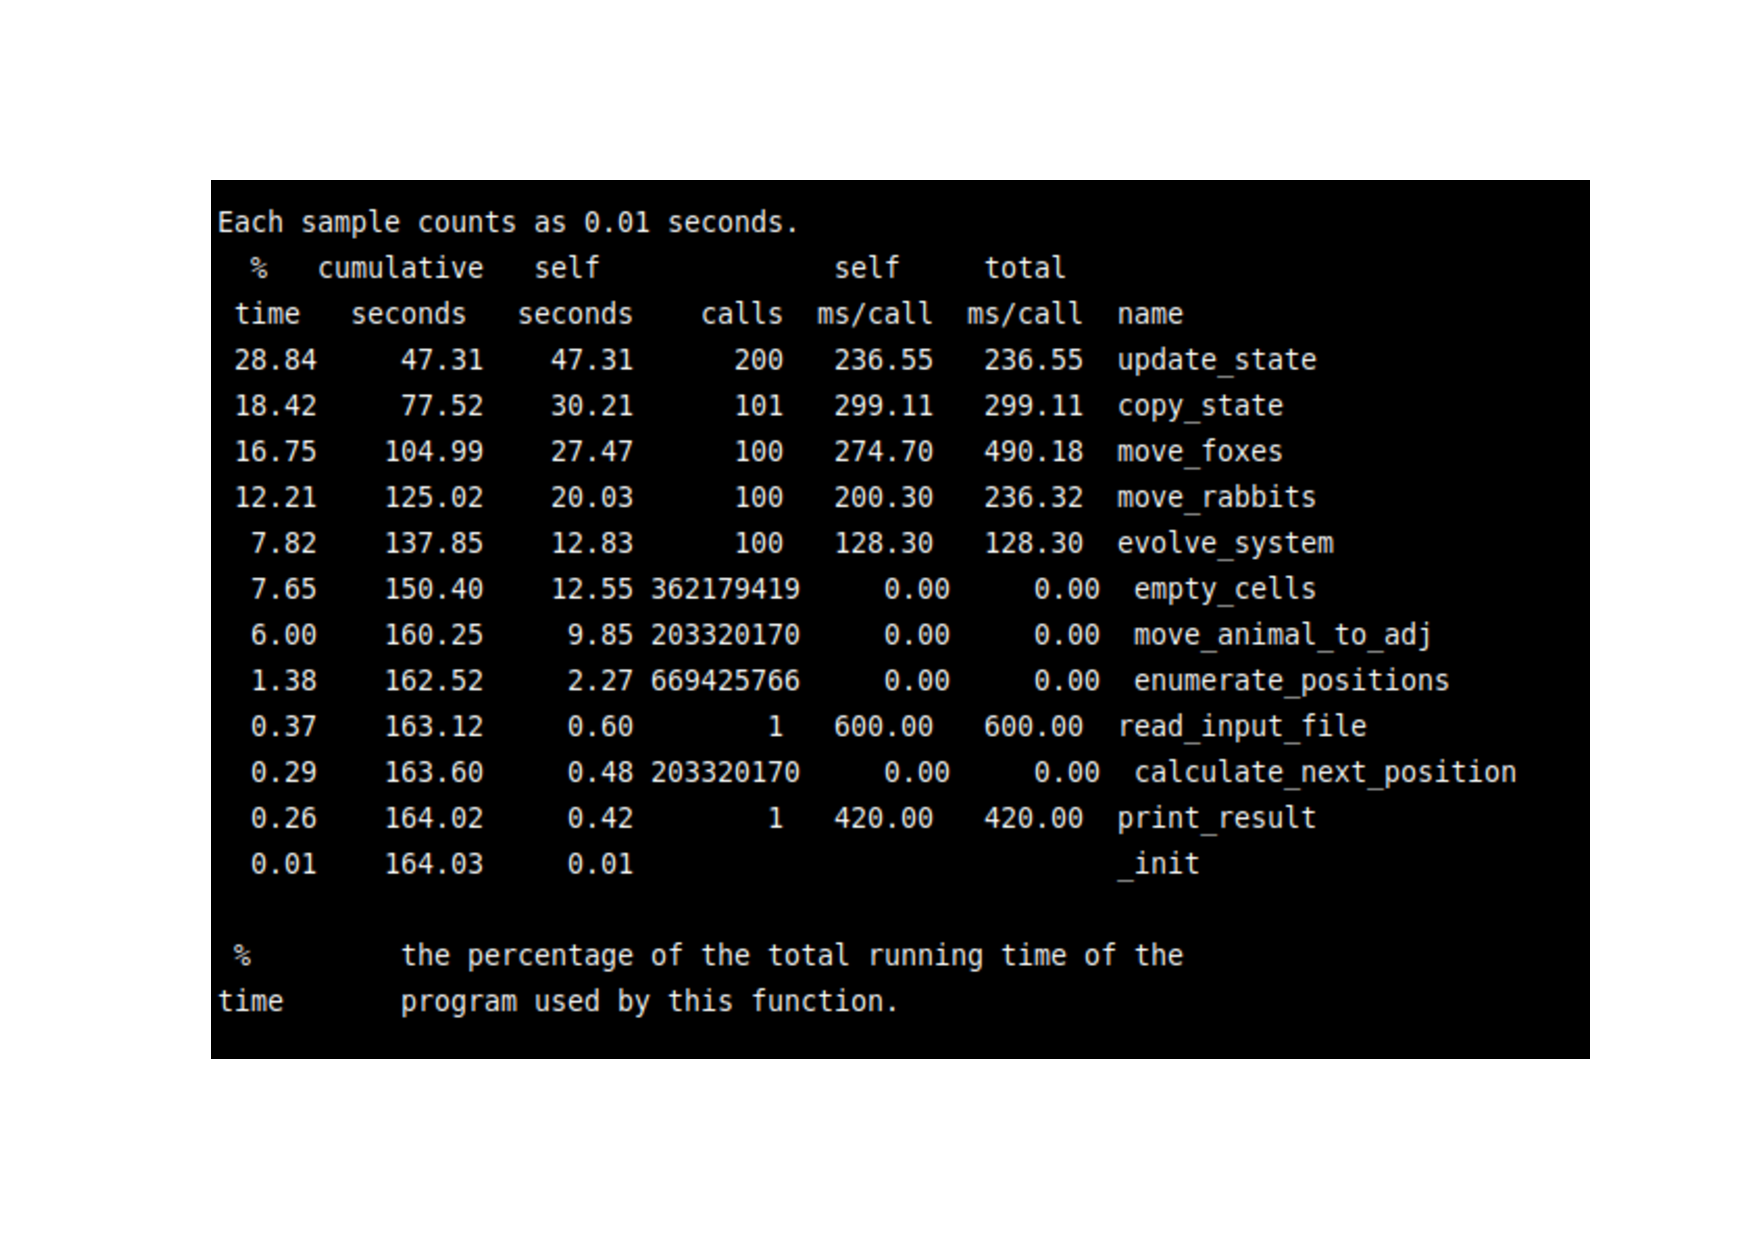
\includegraphics[width=1.1\textwidth]{Images/gprof.pdf}
    \vspace*{-1.5cm}
    \caption{Relatório gerado com a instância \emph{instance\_4.txt}}
    \label{fig:map7}
\end{figure}

O restante do tempo de processamento é dividido entre as funções de movimento de coelhos e raposas, enumeração das posições adjacentes disponíveis e evolução do sistema (20\%, 10\%, 10\% e 10\% aproximadamente, respectivamente). A função responsável pela evolução do sistema apenas percorre a matriz \textbf{A} incrementando o tempo sem procriar dos animais e eliminando raposas que atingiram o limiar de fome.

\subsection{Identificação das Oportunidades de Paralelização}

Como as funções de cópia e atualização das matrizes e de evolução do sistema juntas correspondem em média a aproximadamente 60\% do tempo total de processamento com as instâncias geradas, estas foram as primeiras analisadas como oportunidades para paralelização. Um aspecto em comum entre todas estas funções, é que estas executam apenas operações pontuais em cada célula das matrizes sem que exista quaisquer dependências de dados em relação a quaisquer outras células da matriz (problema embaraçosamente paralelo).

Neste caso, podemos realizar uma decomposição simples de domínio por linhas, colunas, submatrizes ou até mesmo escalonamento de célula por célula para cada \emph{thread} na tentativa de atender requisitos como balanceamento de carga. No caso da função de cópia por exemplo, dado que existe um processador com \(r \times c\) núcleos, seria possível realizar a cópia de todos os elementos ao mesmo tempo, com cada \(r \times c\) \emph{threads} realizando a atribuição de um único elemento da matriz.

Por fim, foram analisadas as funções de movimentação dos animais que, embora possuam a resolução de conflitos no caso de dois ou mais tentarem mover-se para a mesma posição, a operação de movimento como um todo possui dependência de dados na análise e atribuições (movimentar um animal corresponde a um cadeia de atribuições condicionadas, e por isso não é uma instrução atômica) entre as células adjacentes de toda posição (X, Y) analisada. Estas dependências levam a criação de seções críticas em certas porções dos códigos responsáveis pela movimentação dos animais para serem executadas de forma sequencial entre as \emph{threads}.

\subsection{Paralelização}

Em todas as porções de código selecionadas para paralelização estamos lidando com operações em uma matriz. Diante disso, o conjunto de diretivas \textit{D = \{\#pragma omp parallel, \#pragma omp for schedule(type, c), \#pragma omp for, \#pragma omp critical\}} foram utilizadas para introduzir o paralelismo ao programa.

As estratégias utilizadas na paralelização são bastante simples. Nas cinco funções paralelizadas, foi realizada uma decomposição de domínio por linhas da matriz de forma não cíclica. Em outras palavras, para uma matriz de ecossistema com \emph{R} linhas e \emph{N} \emph{threads}, a matriz seria dividida em blocos, com cada bloco contendo possivelmente \emph{N} linhas da matriz, ou seja, a cada bloco, cada \emph{thread} executaria operações em uma linha completa da matriz.

Para as funções \emph{copy\_state}, \emph{update\_state} e \emph{evolve\_system}, utilizou-se apenas a diretiva \textit{\#pragma omp for} de forma que cada \emph{thread} realiza operações em uma linha completa da matriz como mencionado anteriormente. Já para as funções \emph{move\_rabbits} e \emph{move\_foxes}, utilizou-se a diretiva \textit{\#pragma omp for schedule}, dividindo a matriz horizontalmente em partes (\(R / N \times C\)) para cada \emph{thread}. No entanto, nas operações de movimentação dos animais na matriz \textbf{A'}, foi introduzida a diretiva \textit{\#pragma omp critical} devido à existência de dependências de dados entre posições adjacentes na mesma.

\section{Compilação e Execução}

\noindent Para compilar e executar o programa sequencialmente sem ou com perfilamento, basta executar os respectivos comandos via terminal:

\begin{center}
    \boxed{\textbf{\large{make sequential}}}\\
    \vspace{0.5cm}
    \boxed{\textbf{\large{make with\_prof}}}
\end{center}

\noindent Para compilar a versão paralelizada do programa, basta executar o seguinte comando via terminal:

\begin{center}
    \boxed{\textbf{\large{make}}}
\end{center}

\noindent Para executar a versão paralelizada do programa, basta executar o seguinte comando via terminal:

\begin{center}
    \boxed{\textbf{\large{make parallel}}}\\
\end{center}

Os parâmetros de execução podem e devem ser alterados no arquivo \emph{Makefile}, alterando o arquivo de teste por exemplo. Também é possível gerar suas próprias instâncias de teste utilizando o \emph{script Python} presente no diretório \emph{instances}. Basta selecionar os parâmetros do estado inicial do ecossistema e executar o seguinte comando como exemplo:

\begin{center}
    \boxed{\textbf{\normal{python3 instance\_generator.py -l 5 -c 5 -gr 2 -gf 4 -hf 3 -n 6 -r 0.1 -f 0.1 -s 0.2}}}
\end{center}

\section{Análise de Resultados}

Os resultados obtidos foram, no geral, bastante distantes das expectativas. Em vez de apresentar reduções nos tempos de execução, o aumento do número de \emph{threads} apenas elevou os resultados mensurados. O motivo por trás deste comportamento atípico observado na execução paralela do programa ainda não foi descoberto. Todos os testes foram realizados em um computador com processador Intel© Core™ i5-8265U CPU que possui 4 núcleos, 8 \emph{threads} (Hyper-threading) e frequência base 1,60 GHz.

As informações sobre cada instância gerada para teste são apresentadas na Tabela \ref{tab:exampleTab1}. Os parâmetros \emph{rabbits}, \emph{foxes} e \emph{stones} correspondem à porcentagem do total de posições na matriz ocupadas pelo objeto.
\begin{table}[H]
    \centering
    \caption{Parâmetros das Instâncias de Teste}
    \label{tab:exampleTab1}
    \vspace{0.2cm}
    \resizebox{1\columnwidth}{!}{
    \begin{tabular}{c|c|c|c|c|c|c|c|c|c}
        \hline
        \textbf{Instância} & \textbf{r} & \textbf{c} & \textbf{rabbit\_gen} & \textbf{fox\_gen} & \textbf{fox\_food} & \textbf{n\_gen} & \textbf{rabbits} & \textbf{foxes} & \textbf{stones}\\
        \hline
        instance\_1.txt & 7 & 10 & 4 & 6 & 3 & 100 & 20\% & 20\% & 10\%\\
        instance\_2.txt & 100 & 120 & 8 & 10 & 7 & 100 & 20\% & 20\% & 20\%\\
        instance\_3.txt & 500 & 400 & 17 & 20 & 15 & 100 & 30\% & 20\% & 20\%\\
        instance\_4.txt & 5000 & 5000 & 5 & 10 & 15 & 100 & 12\% & 16\% & 8\%\\
        \hline 
    \end{tabular}
    }
\end{table}

\vspace*{-0.5cm}
\begin{figure}[H]
    \centering
    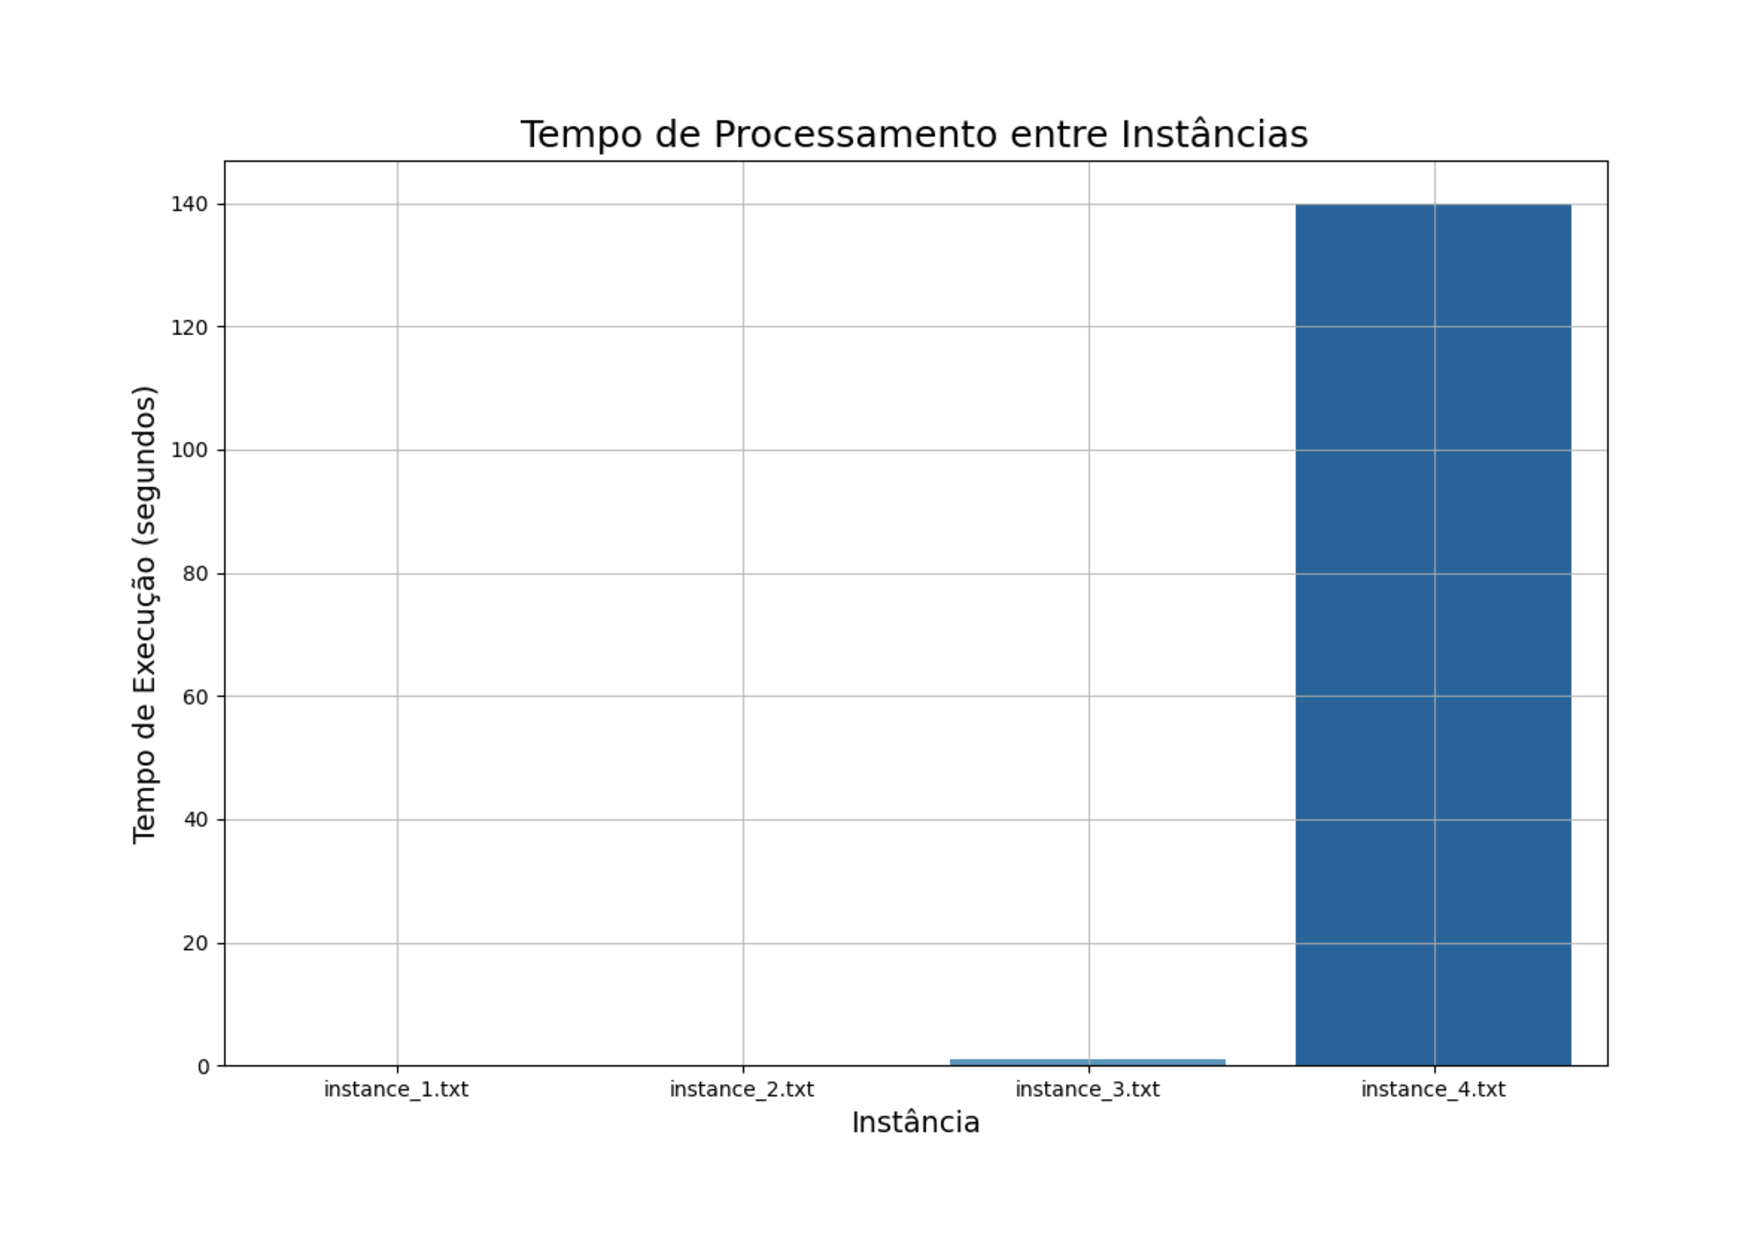
\includegraphics[width=1.1\textwidth]{Images/sequential.pdf}
    \vspace*{-1.5cm}
    \caption{Tempo de execução sequencial}
    \label{fig:map1}
\end{figure}

Na Figura \ref{fig:map1}, podemos observar que o tempo de execução cresce rapidamente conforme os tamanhos do ecossistema crescem (dimensões da matriz), um comportamento dentro do esperado.

Partindo para os resultados obtidos com execuções em paralelo, foram realizados vários testes com quatro valores distintos para o número de \emph{threads} com todas as instâncias. Foram realizados testes com 2, 3 e 4 \emph{threads}, além também do valor máximo (8) para observar como o programa OpenMP lida com a tecnologia de \emph{Hyper-threading} por curiosidade.

Para a primeira instância, como a dimensão do ecossistema é relativamente pequena, não ocorreram diferenças significativas nos tempos de execução mensurados. O gráfico que apresentam as curvas de tempo de processamento para tal instância é apresentado na Figura \ref{fig:map2}.

Para o restante das instância, é possível observar um padrão quanto ao aumento de número de \emph{threads} e o tempo de execução associado. No entanto, os resultados obtidos foram inesperados como mencionado anteriormente, com o tempo de execução aumentando linearmente (diretamente proporcional ao número de \emph{threads}). Os gráficos que apresentam as curvas de tempo de processamento para tais instâncias são apresentados na Figura \ref{fig:map3}, \ref{fig:map4} e \ref{fig:map5}. Por fim, podemos observar na Figura \ref{fig:map6} o quadro geral das execuções sequenciais e em paralelo, com diferentes números de \emph{threads} e instâncias distintas.
\begin{figure}[H]
    \centering
    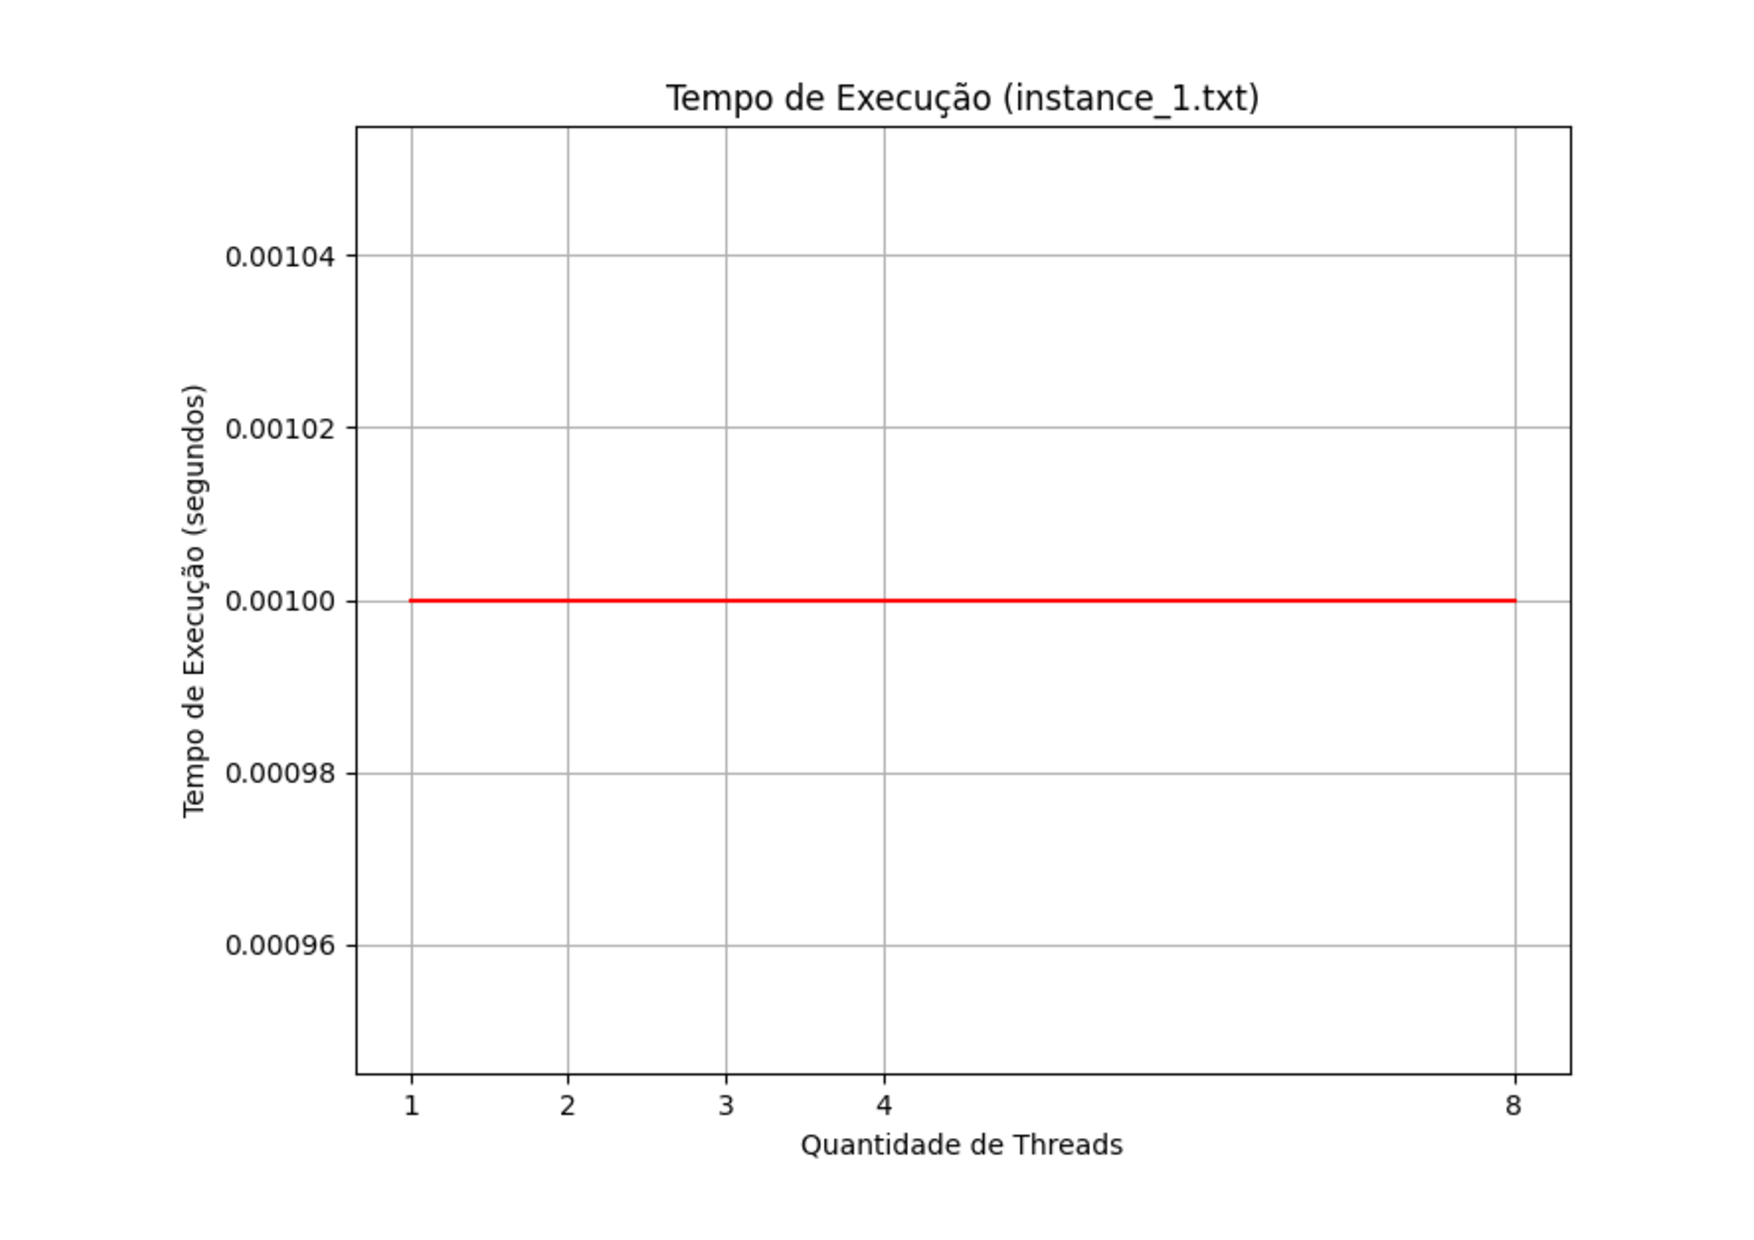
\includegraphics[width=1\textwidth]{Images/instance_1.pdf}
    \vspace*{-1.5cm}
    \caption{Tempos de execução com a instância \emph{instance\_1.txt}}
    \label{fig:map2}
\end{figure}

\begin{figure}[H]
    \centering
    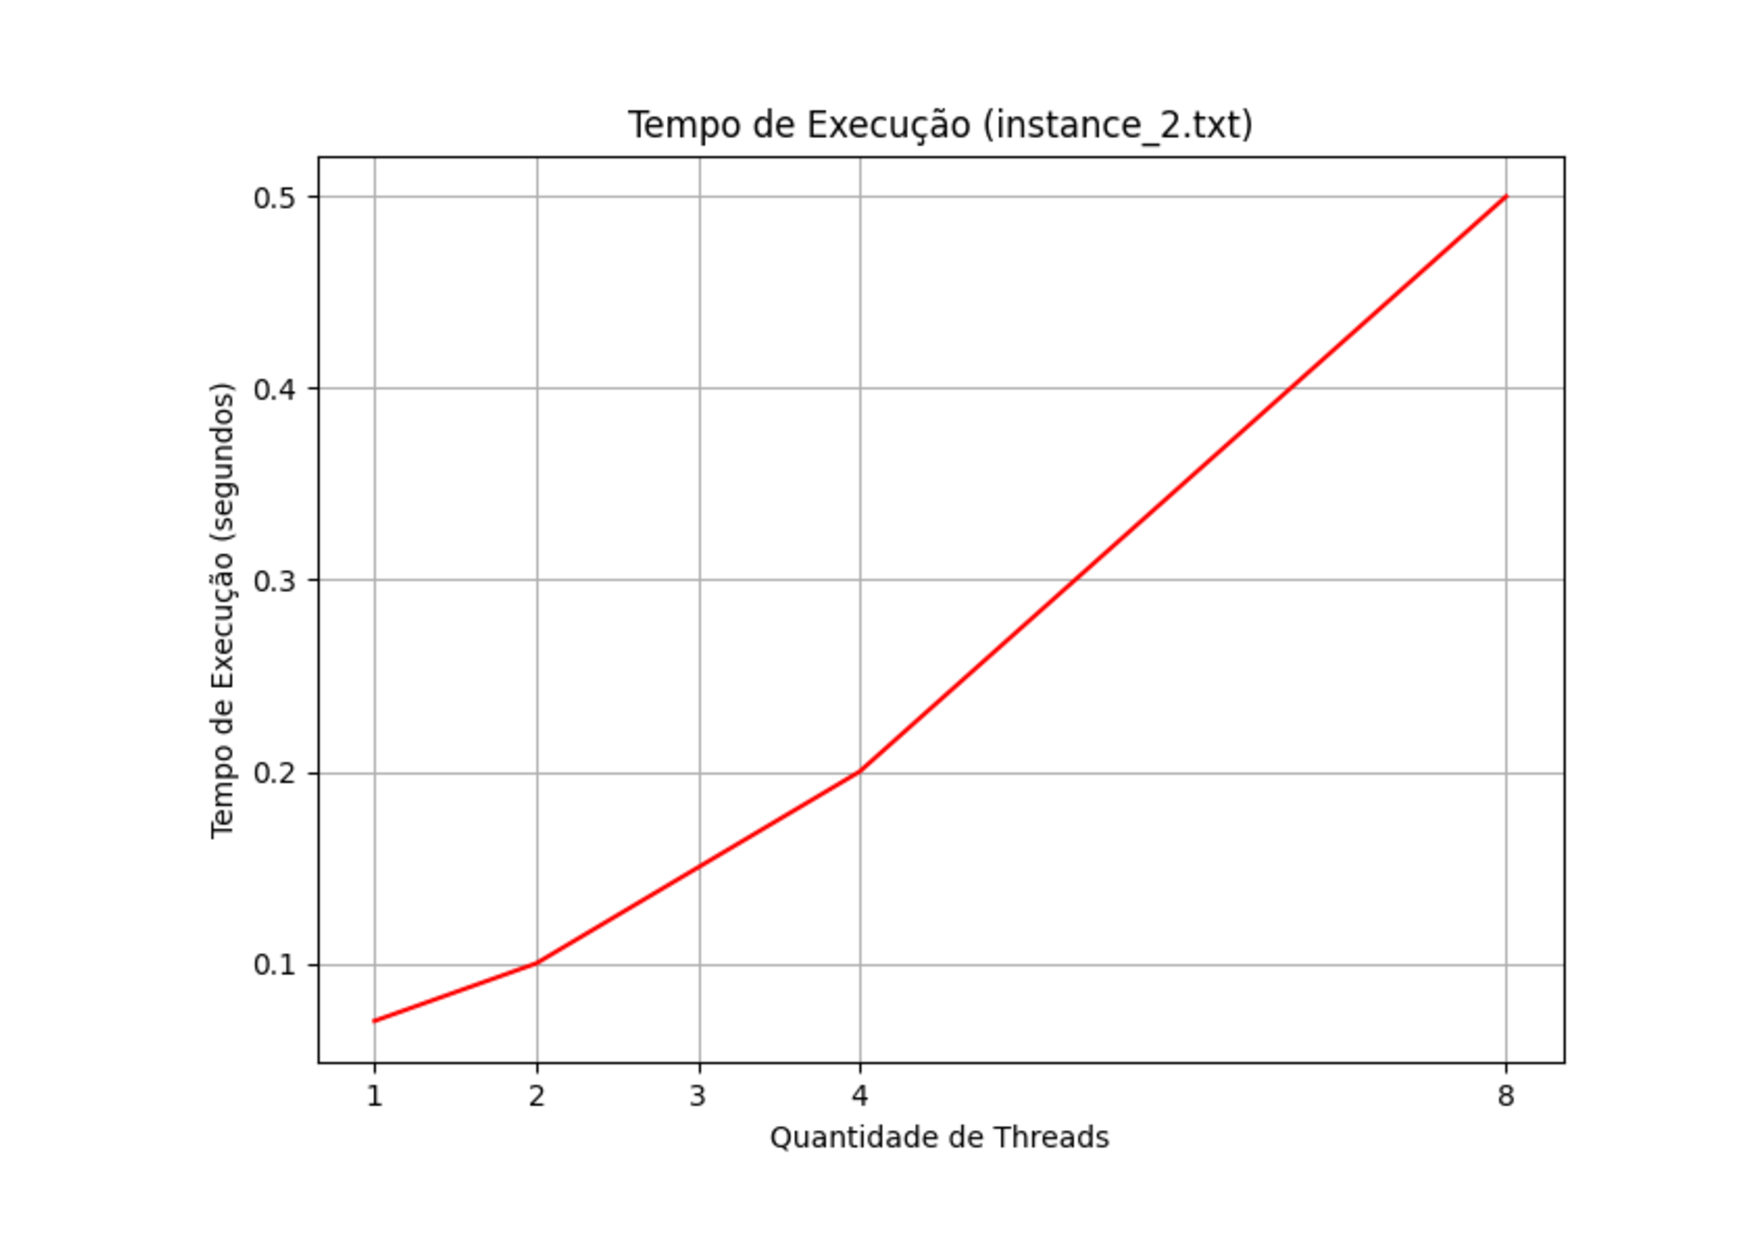
\includegraphics[width=1\textwidth]{Images/instance_2.pdf}
    \vspace*{-1.5cm}
    \caption{Tempos de execução com a instância \emph{instance\_2.txt}}
    \label{fig:map3}
\end{figure}

\begin{figure}[H]
    \centering
    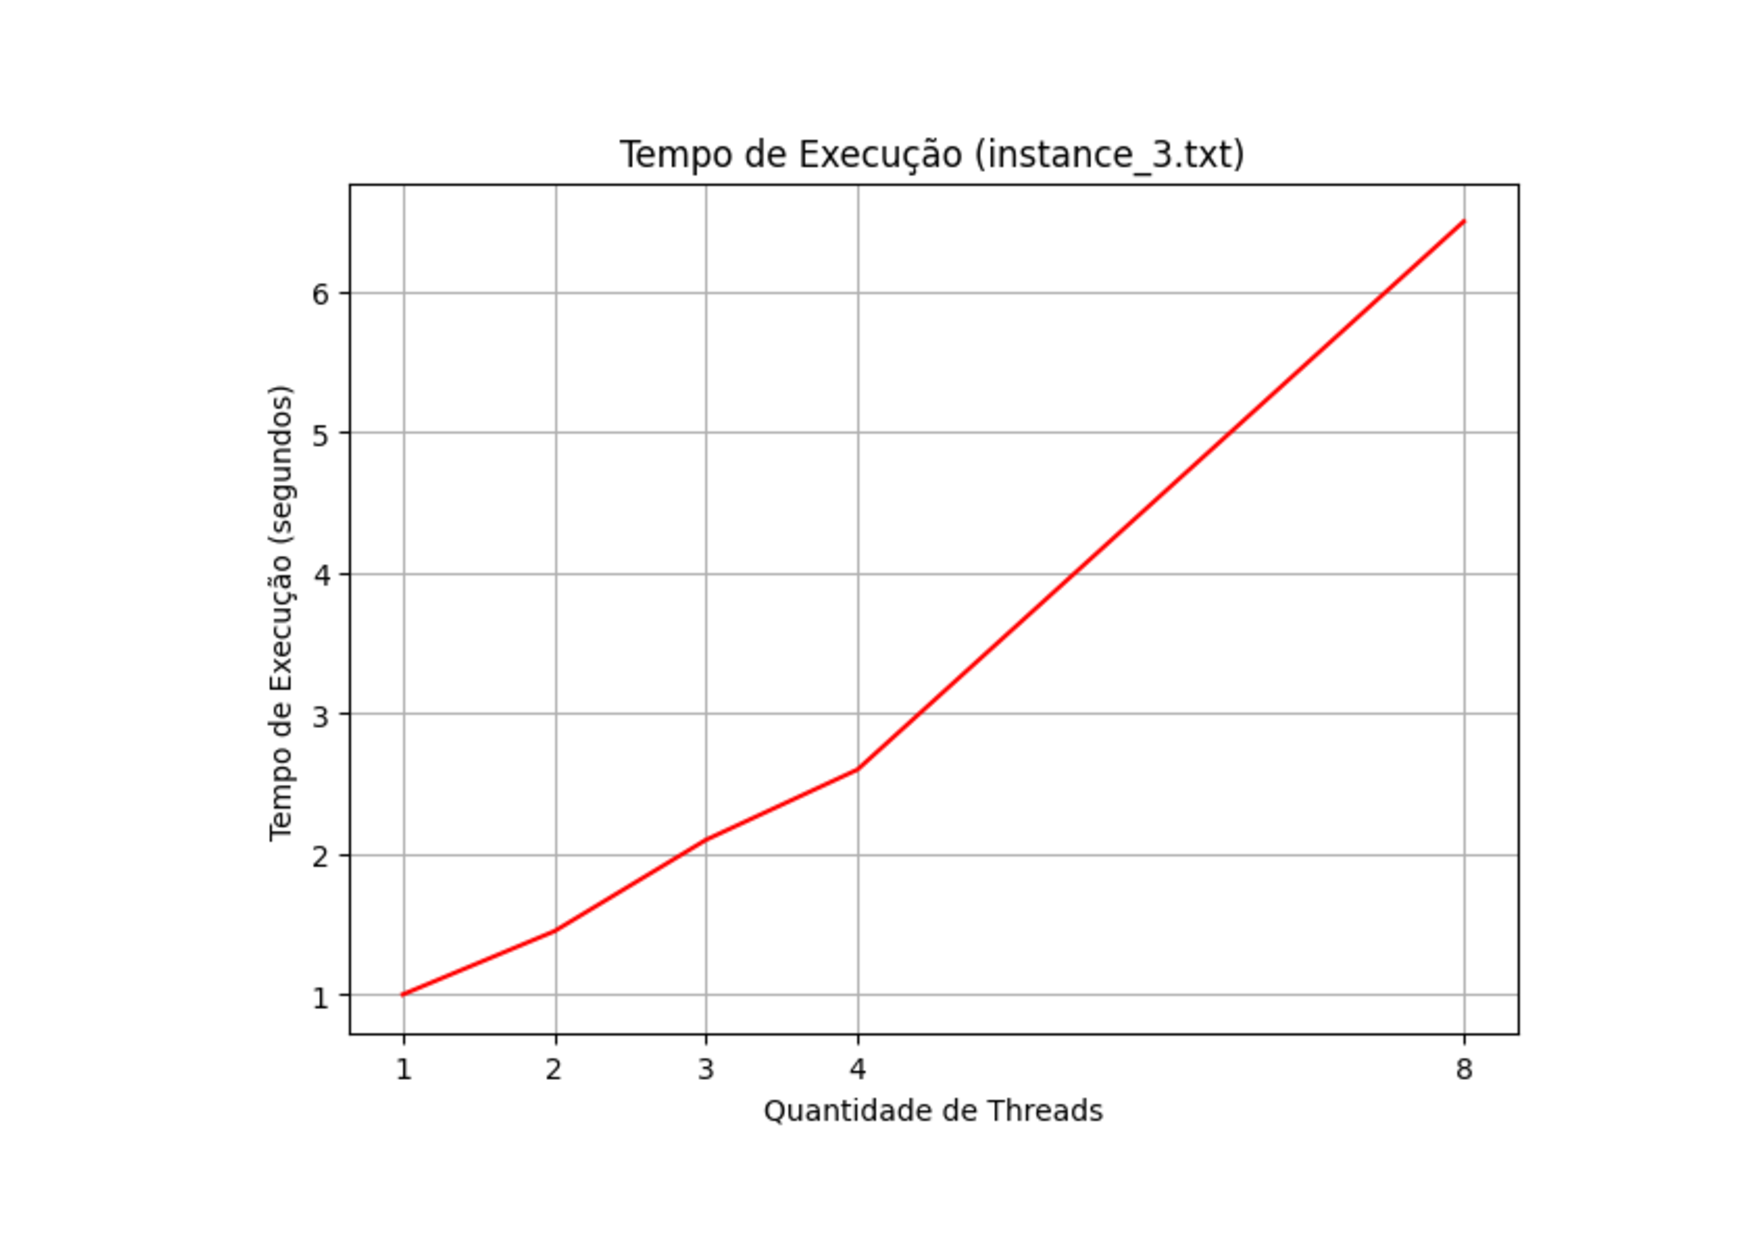
\includegraphics[width=1\textwidth]{Images/instance_3.pdf}
    \vspace*{-1.5cm}
    \caption{Tempos de execução com a instância \emph{instance\_3.txt}}
    \label{fig:map4}
\end{figure}

\begin{figure}[H]
    \centering
    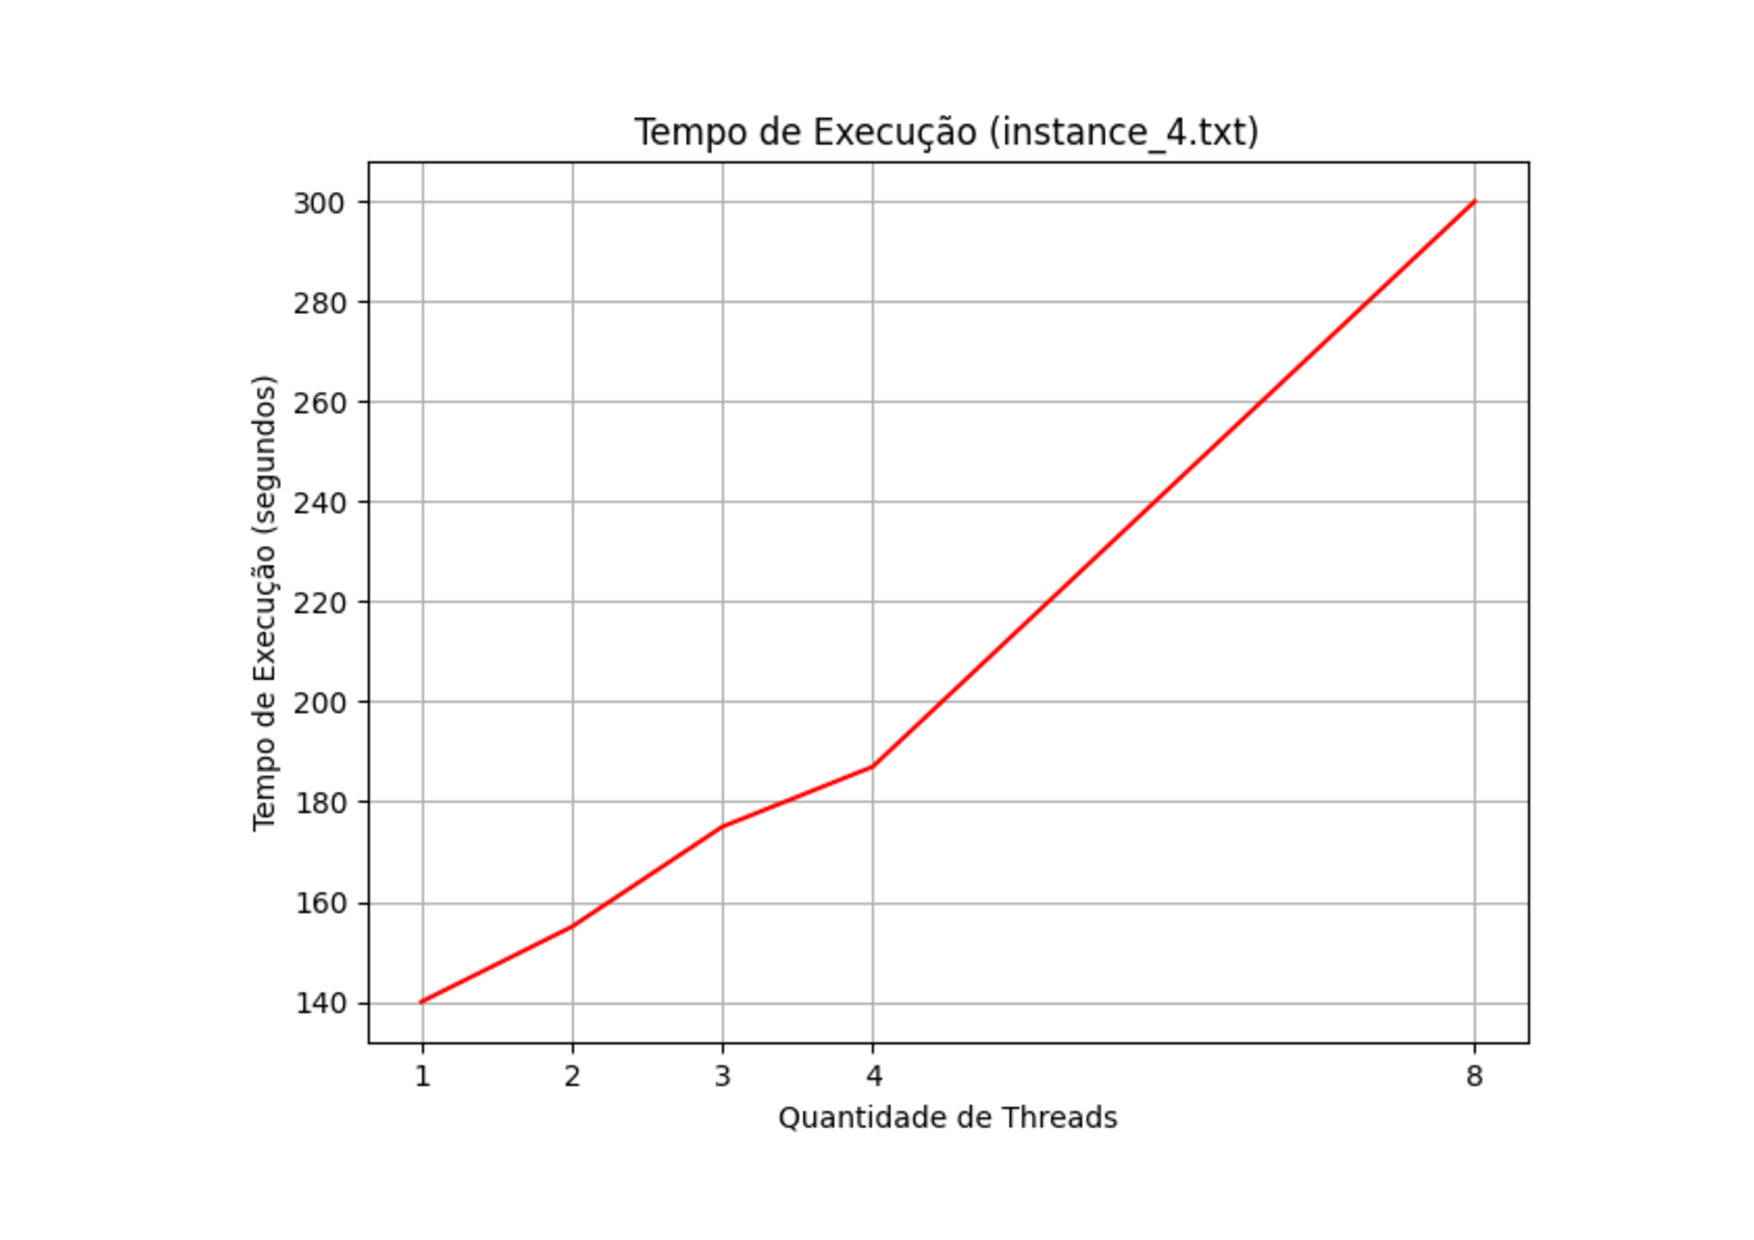
\includegraphics[width=1\textwidth]{Images/instance_4.pdf}
    \vspace*{-1.5cm}
    \caption{Tempos de execução com a instância \emph{instance\_4.txt}}
    \label{fig:map5}
\end{figure}

\vspace*{-1cm}
\begin{figure}[H]
    \centering
    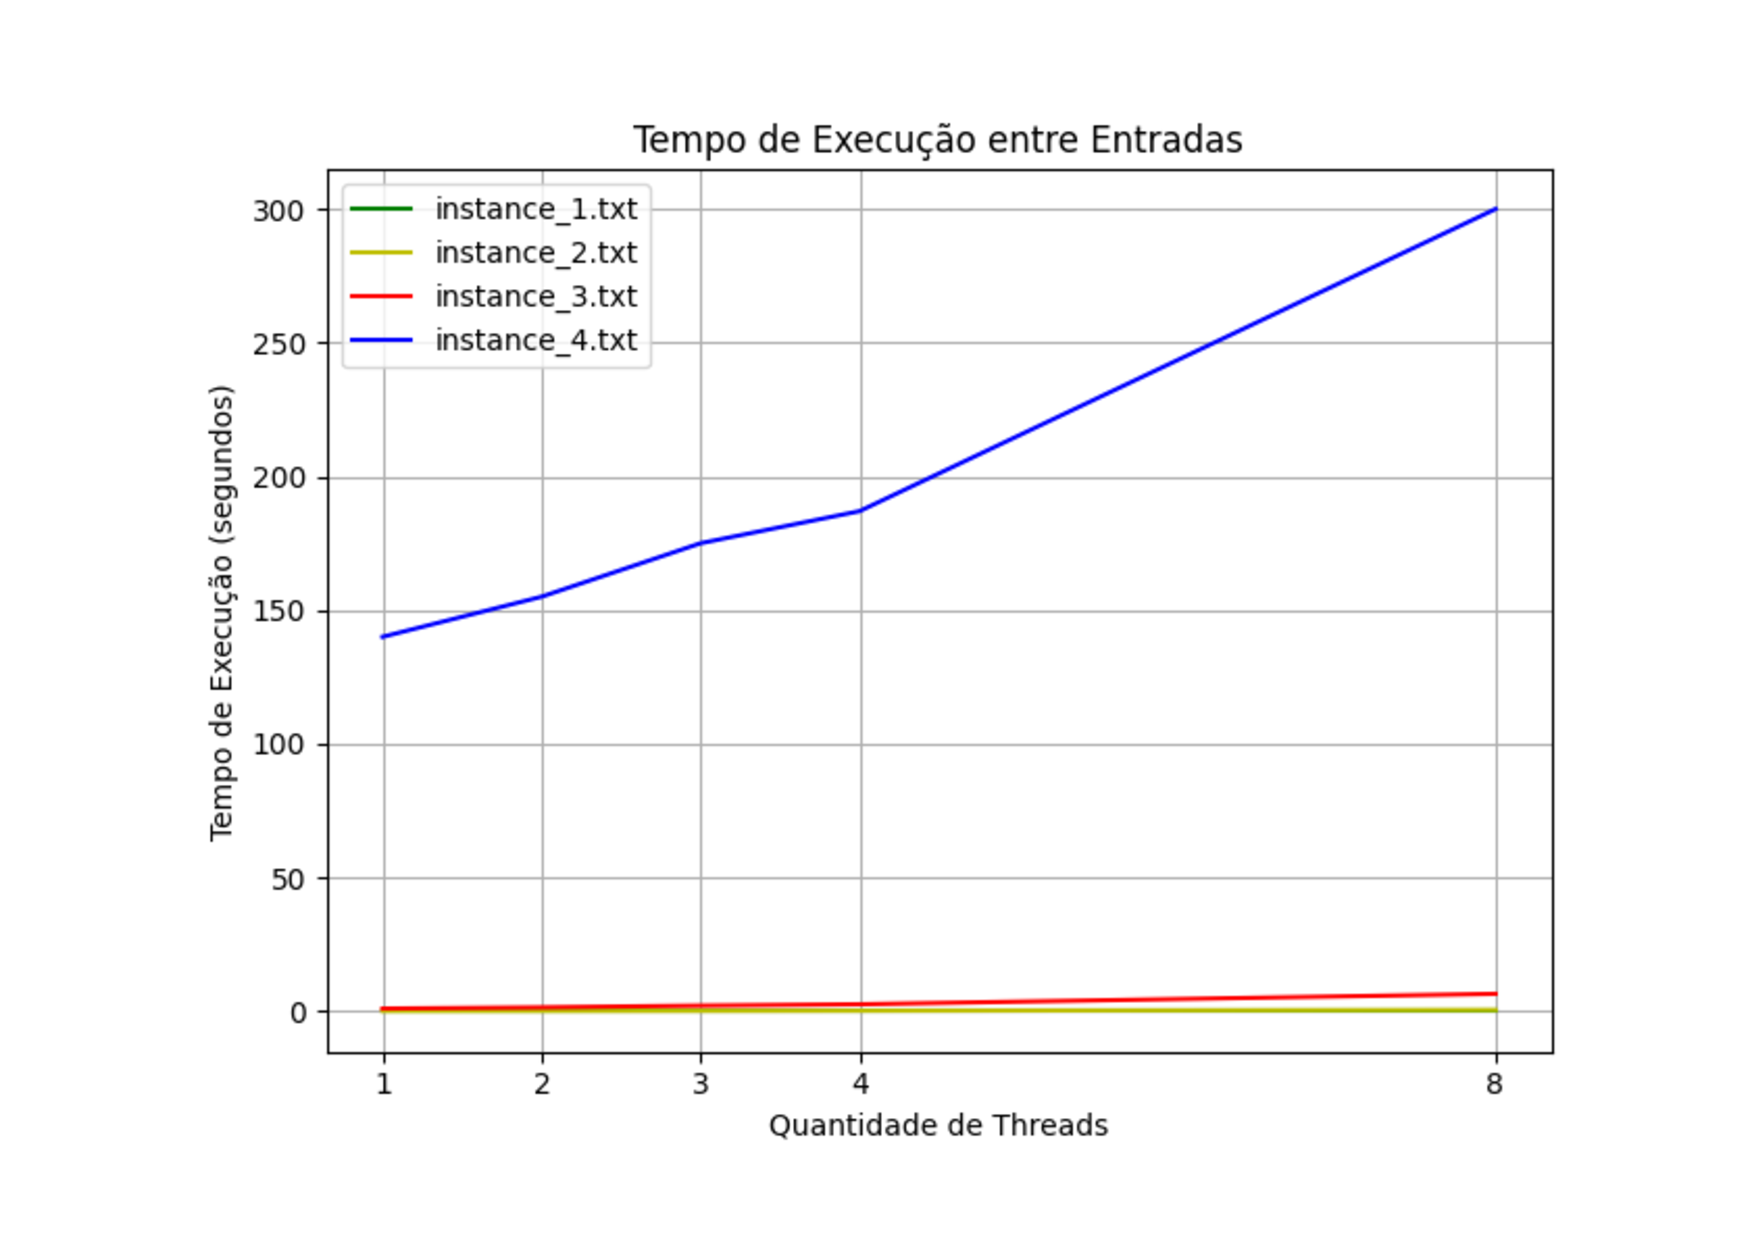
\includegraphics[width=1.1\textwidth]{Images/parallel.pdf}
    \vspace*{-1.5cm}
    \caption{Tempos de execução variando número de \emph{threads} e entradas}
    \label{fig:map6}
\end{figure}

\section{Limitações}

Como principais limitações, é nítido a desvantagem em tempo de processamento entre execuções conforme a quantidade de \emph{threads} aumenta. Seria necessário uma análise mais detalhada de como as diretivas OpenMP estão sendo utilizadas, quais otimizações podem ser feitas para melhorar os resultados ou até se existem erros de implementação que estão provocando a deterioração no tempo de execução.

Além disso, também pode ser de grande relevância analisar como os dados sobre o ecossistema são armazenados. Nesta implementação, por questões de simplificação são utilizadas duas matrizes para manipulá-lo e representá-lo. No entanto, idealmente deveria ser utilizada somente uma matriz para realizar todas as operações, ou até mesmo uma lista, que neste caso, armazenaria somente as posições do ecossistema em que existe um objeto associado (posições vazias não seriam armazenadas).

Refatorações deste tipo possivelmente proveriam uma redução significativa na memória utilizada, principalmente para ecossistemas esparsos (grande quantidade de posições vazias). É importante citar que tais mudanças poderiam também elevar o número de operações necessárias para simulação do ecossistema, possivelmente aumentando o custo computacional em detrimento da menor utilização de armazenamento.

\section{Conclusão}

Neste trabalho, foi explorada uma abordagem de computação paralela para ambiente de memória compartilhada utilizando a biblioteca OpenMP para um problema bastante simples, mas no qual foi possível explorar conceitos como decomposição de domínio e paradigmas SMPD (Single Program Multiple Data).

Com este exemplo didático, podemos observar de forma nítida, a complexidade por trás de construir um programa que será executado em todas as \emph{threads} de forma indiscriminada. Por isto, sempre é necessário ter extrema cautela no controle de dependências de dados e regiões de risco (críticas) entre as \emph{threads}, assim como a alocação e o acesso à memória realizado por cada um.

\pagebreak
\section*{Referências}

\begin{itemize}
    \item Parallel Programming with OpenMP: \url{https://web.njit.edu/~shahriar/class_home/HPC/omp3.pdf};
    \item OpenMP Programming: \url{https://www.cs.cmu.edu/afs/cs/academic/class/15418-s21/www/lectures/rec_04.pdf};
    \item Profiling Programs With prof, gprof, and tcov: \url{https://docs.oracle.com/cd/E19059-01/stud.10/819-0493/OtherTools.html};
    \item Unions: \url{https://www.learn-c.org/en/Unions};
    \item Working with a union of structs in C: \url{https://stackoverflow.com/questions/20752551/working-with-a-union-of-structs-in-c};
    \item Material disponível no SIGAA na disciplina de Computação Paralela.
\end{itemize}

\end{document}